\chapter{D-RI5CY - Vulnerability Assessment}
\chaptermark{D-RI5CY - Vulnerabilities Assessment}
\label{chapter:dift_assessment}
\minitoc

This chapter provides the background of this thesis and the vulnerability assessment. The first section offers a description of the RISC-V Instruction Set Architecture (ISA) and an overview of the specific RISC-V DIFT design under consideration.
The second section details and describes the considered uses cases of this thesis.
Finally, the third section assesses the vulnerabilities of the D-RI5CY, using these three cases.

%%%%%%%%%%%%%%%%%%%%%%%%%%%%%%%%%%%%%%%%%%%%%%%%%%%%%%%%%%%%%%%%%%%%%%%%%%%%%%%%%%%%%%%%%%%%%%%
\section{D-RI5CY}
\label{section:driscy}
In this section, we describe the RISC-V ISA and detail the DIFT design we have chosen to focus on.
We choose to work on RISC-V core as they are open-source, and it means that we have the ability to access and modify the design according to our needs.

\begin{figure}[t]
    \centering
    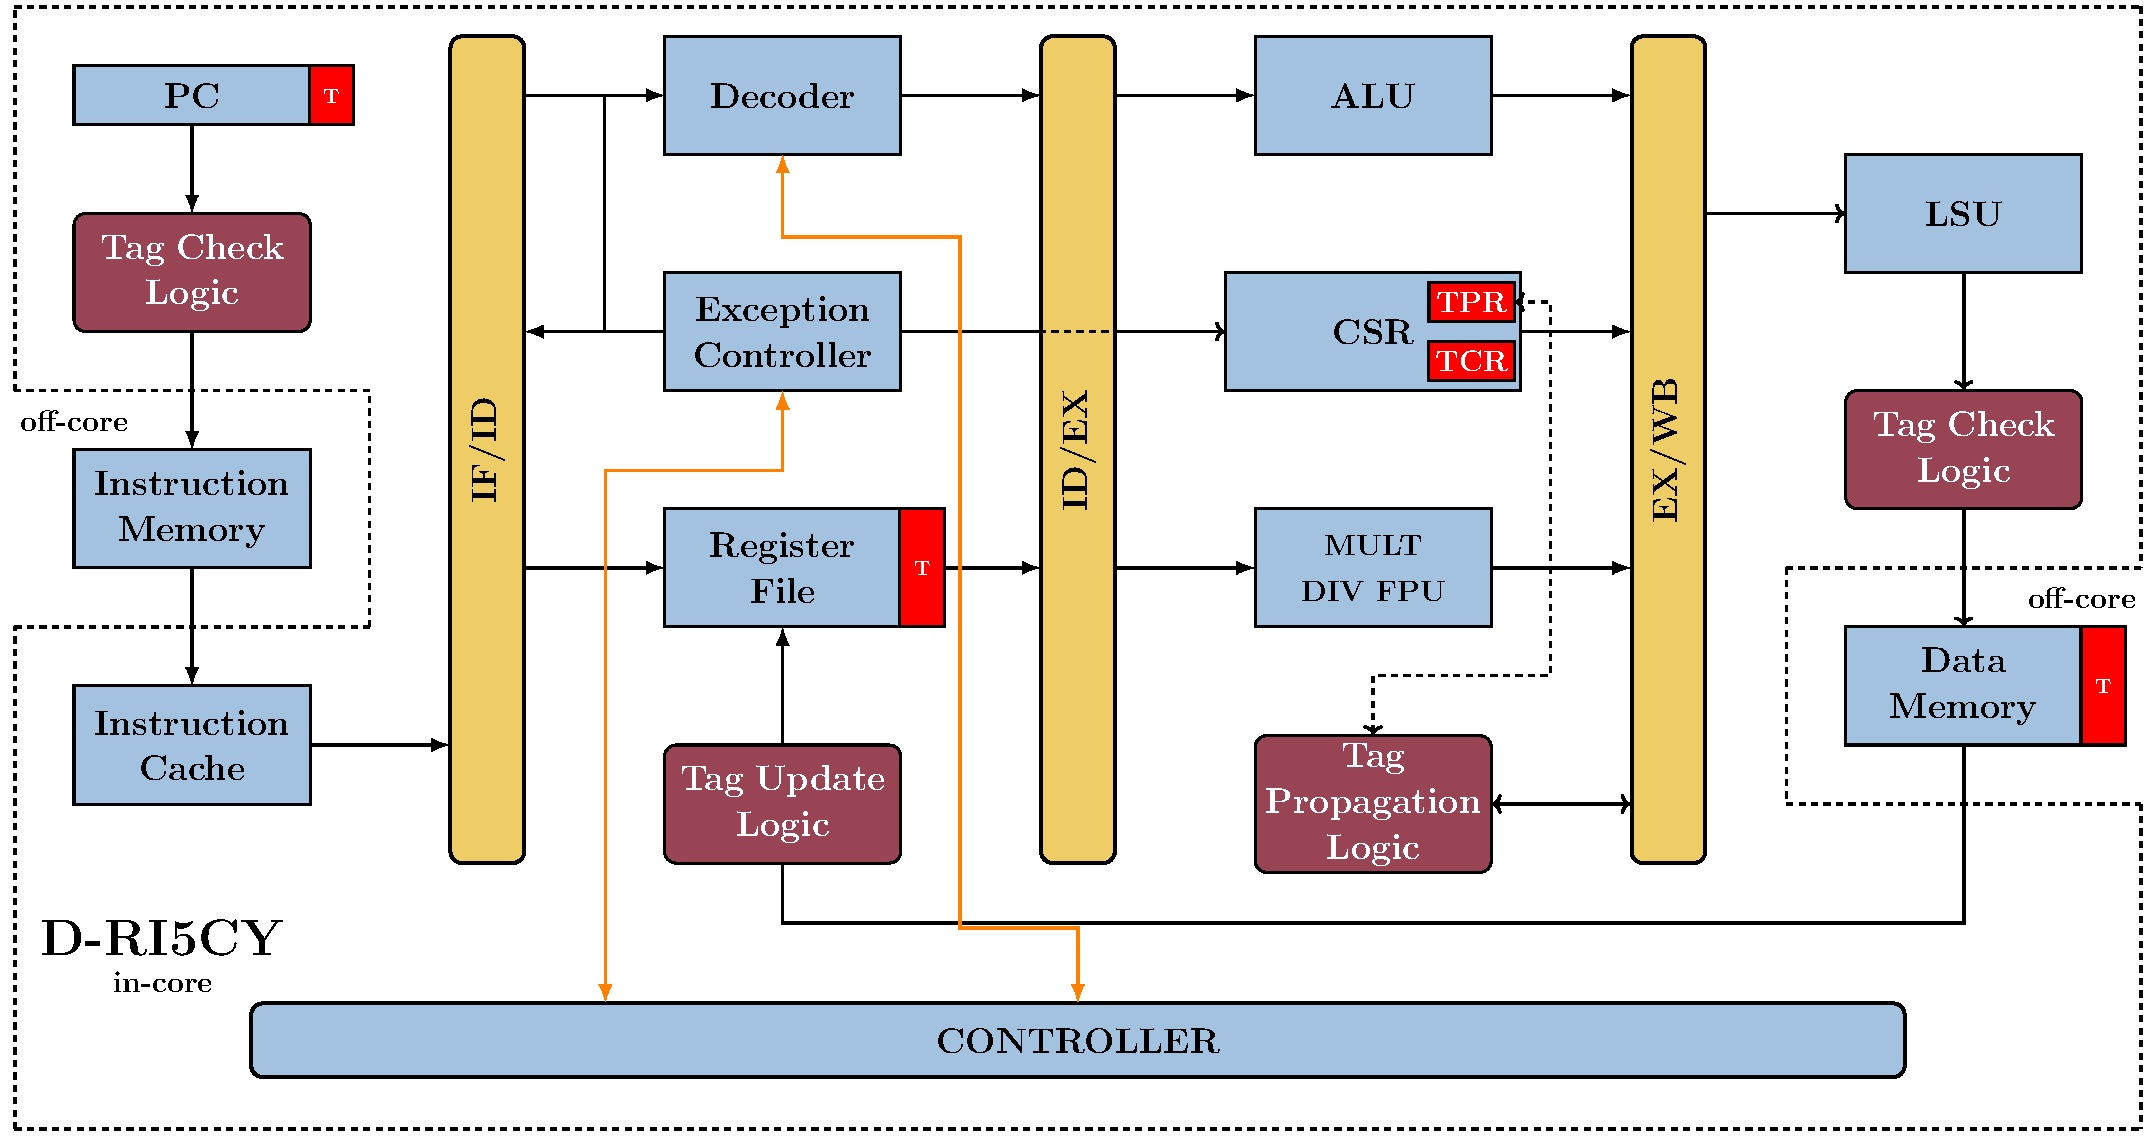
\includegraphics[width=\textwidth]{c3_vulnerabilities_assessment/img/RI5CY.pdf}
    \caption{D-RI5CY processor architecture overview. DIFT-related modules are highlighted in red.}
    \label{fig:driscy}
\end{figure}

%%%%%%%%%%%%%%%%%%%%%%%%%%%%%%%%
\subsection{RISC-V Instruction Set Architecture (ISA)}
RISC-V is an open and free ISA, which was originally developed at University of California, Berkeley, in 2010, and now is managed and supported by the RISC-V Foundation, having more than 70 members including companies such as Google, AMD, Intel, etc. The architecture was designed with a focus on simplicity and efficiency, embodying the Reduced Instruction Set Computer (RISC) principles. Unlike proprietary ISA, RISC-V is freely available for anyone to use without licensing fees, making it a popular choice for academic research, commercial products, and educational purposes.

Technically, RISC-V features a modular design, allowing developers to incorporate only the necessary components for their specific application, which can significantly reduce the processor's complexity and power consumption. It supports several base integer sets classified by width—mainly RV32I, RV64I, and RV128I for 32-bit, 64-bit, and 128-bit architectures respectively. Each base set can be extended with additional modules for applications requiring floating-point computations (e.g., RV32F, RV64F), atomic operations (e.g., RV32A, RV64A), and more. This modularity and the openness of RISC-V have spurred a wide range of innovations in processor design and applications in areas ranging from embedded systems to high-performance computing.

%%%%%%%%%%%%%%%%%%%%%%%%%%%%%%%%
\subsection{DIFT design}
This thesis focus on the evaluation of a DIFT against fault injection attacks in order to protect it. We opted to not develop a Dynamic Information Flow Tracking (DIFT) system from scratch, as this would have required considerable time for implementation and testing, which was not within the scope of our objectives. Consequently, we decided to review the current state of the art and select an open-source DIFT system.
As a result, we have selected the D-RI5CY~\cite{PDGLC-18-hpec, driscy} design, which utilises the RI5CY core supported by PULPino and developed by ETH Zurich. This is a 4-stage, in-order, 32-bit RISC-V core optimised for low-power embedded systems and IoT applications. It fully supports the base integer instruction set (RV32I), compressed instructions (RV32C), and the multiplication instruction set extension (RV32M) of the RISC-V ISA. Additionally, it includes a set of custom extensions (RV32XPulp) that support hardware loops, post-incrementing load and store instructions, and, ALU and MAC operations.

D-RI5CY has been developed by researchers of Columbia University, in the USA, in partnership with Politecnico di Torino, in Italy. D-RI5CY use the RI5CY processor, in which they implemented a hardware in-core DIFT.

Figure~\ref{fig:driscy} presents an overview of the D-RI5CY processor's architecture. In red and dark red are represented the DIFT specific modules.
These modules allow tags to be initialised, propagated and checked during the execution of a sensitive application.
The \textit{Tag Update Logic} module is used to initialize or update the tag in the register file according to the tagged data.
Then, when a tag is propagated in the pipeline in parallel to its associated data, the \textit{Tag Propagation Logic} module propagates it according to the security policy defined in the \textit{TPR}.
Once a tag has been propagated and its data has been sent out of the pipeline, the \textit{Tag Check Logic} modules check that it conforms to the security policy defined in the TCR. If not, an exception is raised and the application is stopped to avoid accessing or executing corrupted data.

The authors of the D-RI5CY defined a library of routines to initialise the tags of the data coming from potentially malicious channels.
At program startup, D-RI5CY initialises the tags of the registers, program counter and memory blocks to \textit{zero}. The default 1-bit tag is "\textit{0}", this means that the data is trusted, otherwise, the tag would be set to "\textit{1}" which means that the data is untrusted.
They extended the RI5CY ISA with memory and register tagging instructions.
They have added four assembly instructions to initialise tags for user-supplied inputs:
\begin{itemize}
    \item \textbf{p.set rd}: sets to untrusted the security tag of the destination register \textit{rd} (you can check the register names in the ISA specification\footnote{\url{https://www2.eecs.berkeley.edu/Pubs/TechRpts/2014/EECS-2014-54.pdf}} at page 85),
    \item \textbf{p.spsb x0, offset(rt)}: sets to untrusted the security tag of the memory byte at the address of the value stored in \textit{rt + offset},
    \item \textbf{p.spsh x0, offset(rt)}: sets to untrusted the security tag of the memory half-word at the address of the value stored in \textit{rt + offset},
    \item \textbf{p.spsw x0, offset(rt)}: sets to untrusted the security tag of the memory word at the address of the value stored in \textit{rt + offset}.
\end{itemize}


Moreover, they augmented the program counter with a tag of one bit and the register file with one tag per register's byte (marked as $T$ in Figure~\ref{fig:driscy}). Finally, they added 4-bit tags to the data memory.
Each data element is physically stored in memory with its associated tag.

It is worth noting that the D-RI5CY designers have chosen to rely on the \textit{illegal instruction exception} already implemented in the original RI5CY processor to manage the DIFT exceptions. This choice minimizes the area overhead of the proposed solution.

In the Control and Status Registers (CSR), they added two additional 32-bits registers : Tag Propagation Register (TPR) and Tag Check Register (TCR). These registers are used to store the security policy for both tag propagation and tag check. These registers contain a default policy, and they can be modified during runtime with a simple \textit{csr write} instruction, such as \texttt{csrw \textit{csr, rs1}}.
These policies consist of rules, which have fine-grain control over tag propagation and tag check for different classes of instructions. The rules specify how the tags of the instruction operands are combined and checked.
Table~\ref{tab:insnClasses} shows the different instructions for each category represented in both TPR and TCR.

\begin{table}[t]
    \centering
    \caption{Instructions per category}
    \label{tab:insnClasses}
    \begin{tabular}{@{}rl@{}}
        \toprule
        \textbf{Class} & \textbf{Instructions} \\ \midrule
        Load/Store & \textit{LW, LH{[}U{]}, LB{[}U{]}, SW, SH, SB, LUI, AUIPC, XPulp Load/Store} \\
        Logical & \textit{AND, ANDI, OR, ORI, XOR, XORI} \\
        Comparison & \textit{SLTI, SLT} \\
        Shift & \textit{SLL, SLLI, SRL, SRLI, SRA, SRAI} \\
        Jump & \textit{JAL, JALR} \\
        Branch & \textit{BEQ, BNE, BLT{[}U{]}, BGE{[}U{]}} \\
        Integer Arithmetic & \textit{ADD, ADDI, SUB, MUL, MULH{[}U{]}, MULHSU, DIV{[}U{]}, REM{[}U{]}} \\ \bottomrule
    \end{tabular}
\end{table}


Table~\ref{tab:tpr} shows the TPR configurations for the security policies considered in our work.
Each instruction type has a user-configurable 2-bit tag propagation policy field, except for \textit{Load/Store Enable}, which has a 3-bit tag. %Each of these field is configured through a write instruction in the CSR.
The tag propagation policy determines how the instruction result tag is generated according to the instruction operand tags.
For 2-bit fields, value `00' disables the tag propagation and the output tag keeps its previous value, value `01' stands for a logic AND on the 2 operand tags, value `10' stands for a logic OR on the 2 operand tags and value `11' sets the output tag to zero. 
The \textit{Load/Store Enable} field provides a finer-granularity rule to enable/disable the input operands before applying the propagation rule specified in the \textit{Load/Store Mode} field. This extra tag propagation policy is defined through 3 bits. These bits allow enabling the source, source-address, and destination-address tags, respectively.

\begin{table}[t]
    \scriptsize
    \setlength{\tabcolsep}{2pt}
    \centering
    \caption{Tag Propagation Register configuration}
    \label{tab:tpr}
    \begin{tabular}{@{}lcccccccc@{}}
        \toprule
                  & \begin{tabular}{c}Load/Store\\Enable \end{tabular} & \begin{tabular}{c}Load/Store\\ Mode
                \end{tabular}  & Logical Mode & Comparison Mode & Shift Mode & Jump Mode & Branch Mode & Arith Mode \\ 
                  \cmidrule(lr){2-2}\cmidrule(lr){3-3}\cmidrule(lr){4-4}\cmidrule(lr){5-5}\cmidrule(lr){6-6}\cmidrule(lr){7-7}\cmidrule(lr){8-8}\cmidrule(lr){9-9}
        Bit index & 17 16 15          & 13 12           & 11 10        & 9 8             & 7 6        & 5 4       & 3 2         & 1 0        \\ \midrule
        Policy 1  & 0 0 1             & 1  0            & 1  0         & 0 0             & 1 0        & 1 0       & 0 0         & 1 0        \\
        Policy 2  & 1 1 1             & 1  0            & 1  0         & 1 0             & 1 0        & 1 0       & 1 0         & 1 0        \\ 
        \bottomrule
    \end{tabular}
\end{table}

Table~\ref{tab:tcr} shows the TCR configurations considered in our work.
Each instruction type has a user-configurable 3-bits tag control policy field, except for \textit{Execute Check}, \textit{Branch Check} and \textit{Load/Store Check} which have 1, 2 and 4-bits tag control policy fields respectively.
The tag control policy determines whether the integrity of the system is corrupted based on the tags of the instruction's operands. 
The default 3-bits field should be read as follows: the right bit corresponds to input operand 1, the middle bit corresponds to input operand 2 and the left bit corresponds to the output tag of the operation. For each bit set, the corresponding tag is checked to determine whether an exception must be raised.
The \textit{Execute Check} field is used to check the integrity of the PC. 
The \textit{Branch Check} field is used to check both inputs during branch instructions. The right bit is used for input operand 1 and the left bit is used for input operand 2.
Finally, the \textit{Load/Store Check} field is used to enable/disable source or destination tags checking during a \textit{load} or \textit{store} instruction. These bits enable or disable the checking of the source tag, source address tag, destination tag and destination address tag.

\begin{table}[t]
    \scriptsize
    \setlength{\tabcolsep}{2pt}
    \centering
    \caption{Tag Check Register configuration}
    \label{tab:tcr}
    \begin{tabular}{@{}lcccccccc@{}}
        \toprule
                  & \begin{tabular}{c}Execute\\Check \end{tabular} & \begin{tabular}{c}Load/Store\\Check \end{tabular}   & Logical Check & Comparison Check & Shift Check & Jump Check & Branch Check & Arith Check \\\cmidrule(lr){2-2}\cmidrule(lr){3-3}\cmidrule(lr){4-4}\cmidrule(lr){5-5}\cmidrule(lr){6-6}\cmidrule(lr){7-7}\cmidrule(lr){8-8}\cmidrule(lr){9-9}
        Bit index & 21            & 20 19 18 17      & 16 15 14      & 13 12 11         & 10 9 8      & 7 6 5      & 4 3          & 2 1 0       \\ \midrule
        Policy 1   & 1             & 1 0 1 0          & 0 0 0         & 0 0 0            & 0 0 0       & 0 0 0      & 0 0          & 0 0 0       \\
        Policy 2 & 0             & 0 0 0 0          & 0 0 0         & 0 0 0            & 0 0 0       & 0 0 0      & 0 0          & 0 1 1       \\
        \bottomrule
    \end{tabular}
\end{table}

To summarise, at first~\textcircled{\small{1}}, D-RI5CY initialises the configuration registers (TPR and TCR) from the default security policy.
Then at program startup~\textcircled{\small{2}}, D-RI5CY initialises all the tags to \textit{trusted} (i.e, set to 0).
The tag propagation~\textcircled{\small{3}} and verification~\textcircled{\small{4}} happen in the D-RI5CY pipeline in parallel with the standard behaviour, without incurring any latency overhead.

%%%%%%%%%%%%%%%%%%%%%%%%%%%%%%%%
\subsection{Pedagogical case study}
To present the use of the D-RISCY, we will introduce a use case to demonstrate how to use a new security policy and how the DIFT will detect the violation of different security policies.
This use case has been developed for pedagogical purposes but does not involve a real software attack.

Listing~\ref{code:compcompu} shows the C code used for this use case. Lines 2 to 4 initialize variables, lines 5 and 6 configure a security policy by writing in the TPR and TCR registers thanks to an assembly line. Line 7 tags the variable "\verb|a|" as untrusted (tag is set to "\textit{1}"). In line 8, variables "\verb|a|" and "\verb|b|" are compared to determine which arithmetic operation should be performed.
Lines 9 to 21 detail the assembly code generated from the line 8 C statement. It executes the operations according to the values of "\verb|a|" and "\verb|b|" stored in the registers "\verb|a4|" and "\verb|a5|". The "\verb|(a>b)|" condition and its associated branch is computed in line 9, the "\verb|(a-b)|" subtraction in line 14 and the "\verb|a+b|" addition in line 20.

The assembly line in C is constructed from keywords \textit{asm volatile}. The template for this assembly line is: "\textit{asm asm-qualifiers ( AssemblerTemplate : OutputOperands [ : InputOperands [ : Clobbers ] ])}".
So to explain briefly,
 line 7 in Listing~\ref{code:compcompu} is composed of a custom assembly instruction "\texttt{p.spsw}", that takes the "\texttt{x0}" register as target and specifies an address mode using the placeholder "\texttt{0(\%0)}". Finally, \mbox{"\textit{:: "r" (\&a)}"} part specifies the input operand, with "\texttt{r}" indicating that a general-purpose register should be used to hold the address of the variable "\texttt{a}".

In terms of security policy, depending on which one we use in Table~\ref{tab:tpr} and Table~\ref{tab:tcr}, we will have different results of exception.
Security policy 1 propagates the tags with an \textit{OR} logic for five modes (arithmetic, jump, shift, logical, and load/store mode) and enables the propagation of the tag from the source of a load/store.
Security policy 1 checks the tags only for the \textit{Execute Check} (i.e., PC instruction) and for the source address and destination address for a load/store instruction.
In comparison, security policy 2 enables the propagation for all tags and checks tags only for both inputs of arithmetic instructions.
To summarise from our application case, if we use security policy 1, the DIFT will detect the \textit{load} instruction before executing the "\verb|a > b|"
 comparison and raise an exception; whereas if we use security policy 2, the DIFT protection raises an exception when executing the instruction \verb|add a5,a4,a5| (i.e., the "\verb|a+b|" C statement), since variable \verb|a| is untrusted and \verb|b > a|.

\begin{lstlisting}[style=topPosition, caption=Compare/Compute C Code, language=C, label=code:compcompu]
    int main(){
       int a, b = 5, c;
       register int reg asm("x9");
       a = reg;
       asm volatile("csrw 0x700, tprValue");
       asm volatile("csrw 0x701, tcrValue");
       asm volatile("p.spsw x0, 0(\%0);" :: "r" (&a));
       c = (a > b) ? (a-b) : (a+b);
           //42c:   ble a4,a5,448
           //430:   addi a5,s0,-16
           //434:   lw a4,-12(a5)
           //438:   addi a3,s0,-16
           //43c:   lw a5,-4(a3)
           //440:   sub a5,a4,a5
           //444:   j 45c
           //448:   addi a5,s0,-16
           //44c:   lw a4,-12(a5)
           //450:   addi a3,s0,-16
           //454:   lw a5,-4(a3)
           //458:   add a5,a4,a5
           //45c:   sw a5,-24(s0)
       return EXIT_SUCCESS;
    }\end{lstlisting}

In the continuation of this work, this use case will be referred to as \textit{Compare/Compute} and will be utilised as the third case, implementing security policy 2 from Table~\ref{tab:tpr} and Table~\ref{tab:tcr}. The two other use cases will be presented in the following section~\ref{section:uses_cases}.

%%%%%%%%%%%%%%%%%%%%%%%%%%%%%%%%%%%%%%%%%%%%%%%%%%%%%%%%%%%%%%%%%%%%%%%%%%%%%%%%%%%%%%%%%%%%%%%
\section{Use cases}
\label{section:uses_cases}

This section details the considered use cases in our work. The first two use cases come from the original paper~\cite{PDGLC-18-hpec}. The third use case is a home-made case which is used to analyse the different DIFT part not studied in others use cases.

%%%%%%%%%%%%%%%%%%%%%%%%%%%%%%%%%%%%%%%%%%
\subsection{First use case: Buffer Overflow}
The first use case involves exploiting a buffer overflow, potentially leading to a Return-Oriented Programming (ROP) attack\footnote{\url{https://github.com/sld-columbia/riscv-dift/blob/master/pulpino\_apps\_dift/wilander\_testbed/}} and the execution of a shellcode. The attacker exploits the buffer overflow to access the return address (\textit{RA}) register. When the function returns, the corrupted \textit{RA} register is loaded into the \textit{PC} via a \textit{jalr} instruction. This hijacks the execution flow, causing the first shellcode instruction to be fetched from address (\textit{0x6fc}). Due to the DIFT mechanism, the tag associated with the buffer data overwrites the \textit{RA} register tag. As the buffer data is user-manipulated, it is tagged as \textit{untrusted} (tag value = 1). Consequently, when the first shellcode instruction is fetched, the tag associated with the \textit{PC} propagates through the pipeline until the DIFT mechanism detects a violation of the security policy and raises an exception. This attack demonstrates the behaviour of DIFT when monitoring the \textit{PC} tag. This use case employs the first security policy from Table~\ref{tab:tpr} and Table~\ref{tab:tcr}.

To illustrate the use of TCR and TPR registers, we assume that buffer data tags are set to 1 (i.e., \textit{untrusted}) since the user manipulates the buffer.
To detect this kind of attack, it is necessary to ensure the PC integrity by prohibiting the use of untrusted data for this register (i.e., \textit{Execute Check} field of TCR set to 1). Regarding tag propagation configuration, load, and store input operand tags must be propagated to output. Thus, the TPR register \textit{Load/Store Mode} field should be set to value 10 (i.e. destination tag = source tag) and the \textit{Load/Store Enable} field must be set to 001 (i.e., Source tag enabled).

Listing~\ref{code:buffer_overflow} displays the C code for the buffer overflow scenario. The assembly code on line 22 of this listing represents the saving of the register \textit{x8}, which is the \textit{saved register 0} or \textit{frame pointer} register in the RISC-V ISA. Next, the source buffer is filled with A's characters and the shellcode address is appended to the end of this source buffer. Finally, lines 30-33 illustrate the tag initialisation on the source buffer.

% \wip{Revoir cette partie avec nouvelle version de l'image}
Figure~\ref{fig:rop_attack} represents the five steps from the source buffer initialisation to the first shellcode instruction being fetched.
In Figure~\ref{fig:rop_attack_1}, the source buffer, in yellow, is initialised with A's, and as it is manipulated by a user, it is tagged as untrusted (red). The destination buffer is empty, and both \textit{PC} and \textit{RA} register are trusted (green).
In Figure~\ref{fig:rop_attack_2}, the source buffer is copied into the destination buffer, the data and its tag are copied.
In Figure~\ref{fig:rop_attack_3}, the overflow occurs, and the $ra$ register is compromised with the address of the shellcode function from the source buffer. Now, all the memory tags are untrusted.
In Figure~\ref{fig:rop_attack_4}, the \textit{PC} loads the $ra$ register along with its tag. The \textit{PC} loses its integrity and became untrusted.
In Figure~\ref{fig:rop_attack_5}, the \textit{PC} address is fetched, and the instruction is sent into the pipeline along with the tag.
At this moment, the DIFT mechanism will detect the untrusted tag and as the security policy do not allow executing an untrusted PC, an exception will be raised and the application will be stopped.

\begin{lstlisting}[style=topPosition, language=C, label=code:buffer_overflow, caption=Buffer overflow C code]
#define BUFSIZE 16
#define OVERFLOWSIZE 256

int base_pointer_offset;
long overflow_buffer[OVERFLOWSIZE];

int shellcode() {
    printf("Success !!\n");
    exit(0);
}

void vuln_stack_return_addr(){
    long *stack_pointer;
    long stack_buffer[BUFSIZE];
    char propolice_dummy[10];
    int overflow;
    
    /* Just a dummy pointer setup */
    stack_pointer = &stack_buffer[1];
    
    /* Store in i the address of the stack frame section dedicated to function arguments */
    register int i asm("x8");  
    
    /* First set up overflow_buffer with 'A's and a new return address */
    overflow = (int)((long)i - (long)&stack_buffer);
    memset(overflow_buffer, 'A', overflow-4);
    overflow_buffer[overflow/4-1] = (long)&shellcode;

    /* TAG INITIALISATION */
    for(int j=0; j<overflow/4; j++) {
        asm volatile ("p.spsw x0, 0(%[ovf]);"                
                    ::[ovf] "r" (overflow_buffer+j));
    }

    /* Then overflow stack_buffer with overflow_buffer */
    memcpy(stack_buffer, overflow_buffer, overflow); 
    
    return;
}

int main(){
    vuln_stack_return_addr();
    printf("Attack prevented.\n");
    return EXIT_SUCCESS;
}\end{lstlisting}

\begin{figure}[ht]
    \centering
    \begin{subfigure}[b]{0.49\textwidth}
        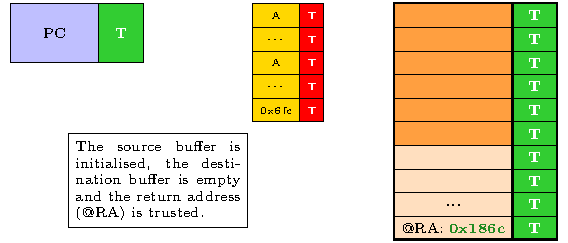
\includegraphics[width=\textwidth, page=1]{c3_vulnerabilities_assessment/img/buffer_overflow/schemaPedagogique.pdf}
        \caption{Initialisation}
        \label{fig:rop_attack_1}
    \end{subfigure}
    \hfill
    \begin{subfigure}[b]{0.49\textwidth}
        \includegraphics[width=\textwidth, page=2]{c3_vulnerabilities_assessment/img/buffer_overflow/schemaPedagogique.pdf}
        \caption{Copy of the source buffer into the destination buffer}
        \label{fig:rop_attack_2}
    \end{subfigure}
    \hfill
    \begin{subfigure}[b]{0.49\textwidth}
        \includegraphics[width=\textwidth, page=3]{c3_vulnerabilities_assessment/img/buffer_overflow/schemaPedagogique.pdf}
        \caption{An overflow occurs, the $ra$ register is overwritten}
        \label{fig:rop_attack_3}
    \end{subfigure}
    \hfill
    \begin{subfigure}[b]{0.49\textwidth}
        \includegraphics[width=\textwidth, page=4]{c3_vulnerabilities_assessment/img/buffer_overflow/schemaPedagogique.pdf}
        \caption{Corrupted $ra$ register is loaded into the PC}
        \label{fig:rop_attack_4}
    \end{subfigure}
    \hfill
    \begin{subfigure}[b]{0.49\textwidth}
        \includegraphics[width=\textwidth, page=5]{c3_vulnerabilities_assessment/img/buffer_overflow/schemaPedagogique.pdf}
        \caption{PC address instruction is fetched}
        \label{fig:rop_attack_5}
    \end{subfigure}
    \caption{Representation of how the ROP attack works}
    \label{fig:rop_attack}
\end{figure}

%%%%%%%%%%%%%%%%%%%%%%%%%%%%%%%%%%%%%%%%%%
\subsection{Second use case: Format String (WU-FTPd)}
The second use case is a format string attack\footnote{\url{https://github.com/sld-columbia/riscv-dift/tree/master/pulpino_apps_dift/wu-ftpd}} overwriting the return address of a function to jump to a shellcode and starts its execution.  This use case uses the first security policy from Table~\ref{tab:tpr} and Table~\ref{tab:tcr}.
This attack exploits the \verb|printf()| function from the C library. It uses the \verb|%u| and \verb|%n| formats (see Chapter 12, Section 12.14.3 in~\cite{gnu_lib_c} for detailed information) to write the targeted address.

Listing~\ref{code:wu_ftpd} shows the C code of this use case. The \texttt{echo} function assign the \textit{x8} register to a variable '\verb|i|' which goes into another variable '\verb|a|'.
The lines 13-14 are used to initialise the tag associated to the variable '\verb|a|'. This variable `\verb|a|' is user-defined, so it is tagged as untrusted for DIFT computation.
The vulnerable statement is the \verb|printf| statement in line 16.
The format \verb|%u| is used to print unsigned integer characters.
The format \verb|%n| is used to store in memory the number of characters printed by the \verb|printf()| function, the argument it takes is a pointer to a signed int value. 

The execution of the \verb|printf| at line 16 leads to write in memory 224 (0xe0) at address (a-4), 224+35 so 259 (0x103) at address (a-3), and 512 (0x200) at addresses (a-2) and (a-1). The attacker's objective is to overwrite the return address with `\textit{0x3e0}' which represent the address of the first function, called \textit{secretFunction} in Listing~\ref{code:wu_ftpd}. In this case, security policy prohibits the use of untrusted variables as store addresses. Since variable `\verb|a|' is untrusted, the DIFT protection raises an exception when storing a value at memory address \verb|(a-4)|. This use case has been chosen to activate the load/store modes of the DIFT policy. 

\begin{lstlisting}[style=topPosition, language=C,label=code:wu_ftpd, caption=WU-FTPd C code]
void secretFunction(){
    printf("Congratulations!\n");
    printf("You have entered in the secret function!\n");

    exit(0);
}

void echo(){
    int a;
    register int i asm("x8");
    a = i;

    asm volatile ("p.spsw x0, 0(%[a]);"                
                ::[a] "r" (&a));

    printf("%224u%n%35u%n%253u%n%n", 1, (int*) (a-4), 1, (int*) (a-3), 1, (int*) (a-2), (int*) (a-1));

    return;
}

int main(int argc, char* argv[]){ 
    volatile int a = 1;

    if(a)
        echo();
    else
        secretFunction();

    return 0;
}\end{lstlisting}

Table~\ref{table:ftpdOverwriteMemory} represents the different steps to overwrite the memory with the exact address of the malicious function. We can see that after each write and the right shift of the writing, the address appears. Finally, we have the address '\textit{000002000003E0}' in memory from 'A+2' to 'A-4' but as an address is on 32-bits in our architecture, the address fetched by the pipeline is only '\textit{000003E0}'.

\begin{table}[t]
    \centering
    \caption{Memory overwrite}
    \label{table:ftpdOverwriteMemory}
    \begin{tabular}{l|ccccccc}
        \toprule
        Address & A-4 & A-3 & A-2 & A-1 & A & A+1 & A+2 \\ \midrule
        A-4     & \textit{0xE0} & \textit{0x00} & \textit{0x00} & \textit{0x00} & \textit{}     & \textit{}     & \textit{}     \\
        A-3     & \textit{}     & \textit{0x03} & \textit{0x01} & \textit{0x00} & \textit{0x00} & \textit{}     & \textit{}     \\
        A-2     & \textit{}     & \textit{}     & \textit{0x00} & \textit{0x02} & \textit{0x00} & \textit{0x00} & \textit{}     \\
        A-1     & \textit{}     & \textit{}     & \textit{}     & \textit{0x00} & \textit{0x02} & \textit{0x00} & \textit{0x00} \\ \midrule
        Memory & {0xE0}    & {0x03}    & 0x00          & 0x00          & 0x02          & 0x00          & 0x00          \\
        \bottomrule
    \end{tabular}
\end{table}


%%%%%%%%%%%%%%%%%%%%%%%%%%%%%%%%%%%%%%%%%%%%%%%%%%%%%%%%%%%%%%%%%%%%%%%%%%%%%%%%%%%%%%%%%%%%%%%
\section{Vulnerability assessment}
\label{section:vuln_assessment}
In order to analyse the behaviour of the processor at application runtime against Fault Injection Attacks, we have simulated some fault injections campaigns in which we inject fault inside the 55 registers associated to the DIFT, which correspond to 127 bits in total. For these campaigns, we use a tool, developed for this purpose. This tool is described in Chapter~\ref{chapter:fissa} and can generate the TCL code to automatise fault injections attacks campaigns at\textit{ Cycle Accurate and Bit Accurate} (CABA) level.
Table~\ref{tab:registersDIFT} shows the repartition of these registers in every pipeline stage of the RI5CY core and the number of associated bits. This work has been published in ACM Sensors S\&P~\cite{PLG-22-SensorsSP}.

\begin{table}[t]
    \centering
    \caption{Numbers of registers and quantity of bits represented}
    \label{tab:registersDIFT}
    \begin{tabular}{@{}ccc@{}}
        \toprule
        \textbf{HDL Module} & \textbf{Number of registers} & \textbf{Number of bits in registers} \\ \midrule
        Instruction Fetch Stage & 2 & 2 \\
        Instruction Decode Stage & 14 & 19 \\
        Register File Tag & 1 & 32 \\
        Execution Stage & 1 & 1 \\
        Control and Status Registers & 2 & 64 \\
        Load/Store Unit & 4 & 9 \\
        \midrule
        \midrule
        \textbf{Total} & \textbf{\textbf{24}} & \textbf{\textbf{127}} \\
        \bottomrule
    \end{tabular}
\end{table}

We assess the design with fault injection campaigns. With their results associated, we can deduce which registers are vulnerable with the cycle associated and the fault model. This assessment is done for each use case for a more precise analysis and to understand how the tag is propagated and checked before the exception.

%%%%%%%%%%%%%%%%%%%%%%%%%%%%%%%%%%%%%%%%%%
\subsection{Fault model for vulnerability assessment}
In this vulnerability assessment, we consider an attacker able to inject faults into DIFT-related registers leading to \textit{set to 0}, \textit{set to 1}, and \textit{single bit-flip in one register at a given clock cycle}. To bypass the DIFT mechanism, the main attacker's goal is to prevent an exception being raised. To reach this objective, any DIFT-related register maintaining tag value, driving the tag propagation or the tag update process or maintaining the security policy configuration can be targeted.


%%%%%%%%%%%%%%%%%%%%%%%%%%%%%%%%%%%%%%%%%%
\subsection{First use case: Buffer overflow}
Table~\ref{tab:end_sim_from_time_fault_register_bo} shows that 22 fault injections in four different DIFT-related registers can lead to a successful attack despite the DIFT mechanism (i.e., DIFT protection is bypassed). 
For example, it shows that a fault injection targeting the~\textit{pc\_if\_o\_tag} register can defeat the DIFT protection if a fault is injected at cycle 3431 using a bit-flip or a set to 0 fault type.
Furthermore, Table~\ref{tab:end_sim_from_time_fault_register_bo} shows that five different cycles can be targeted for the attack to succeed. In most cases, \textit{bit-flip} leads to a successful injection with 11 successes over 22. Faults in \textit{tpr\_q} and \textit{tcr\_q} are successful, since these registers maintain the propagation rules and the security policy configuration (see Table~\ref{tab:tpr} and Table~\ref{tab:tcr} for more details about each bit position). Both \textit{pc\_if\_o\_tag} and \textit{rf\_reg[1]} are also critical registers for this use case. Indeed, \textit{pc\_if\_o\_tag} allows the propagation of the PC tag while \textit{rf\_reg[1]} stores the tag of the return address register $ra$.

\begin{table}[t]
    \small
    \centering
    \setlength{\tabcolsep}{4pt}
    \caption{Buffer overflow: success per register, fault type and simulation time}
    \label{tab:end_sim_from_time_fault_register_bo}
    \begin{tabular}{@{}lccccccccccccccc@{}}
        \toprule
         & \multicolumn{3}{c}{Cycle 3428} & \multicolumn{3}{c}{Cycle 3429} & \multicolumn{3}{c}{Cycle 3430} & \multicolumn{3}{c}{Cycle 3431} & \multicolumn{3}{c}{Cycle 3432} \\\cmidrule(lr){2-4}\cmidrule(lr){5-7}\cmidrule(lr){8-10}\cmidrule(lr){11-13}\cmidrule(lr){14-16}
         & set0 & set1 & bit-flip & set0 & set1 & bit-flip & set0 & set1 & bit-flip & set0 & set1 & bit-flip & set0 & set1 & bit-flip \\
        \midrule
        pc\_if\_o\_tag &  &  &  &  &  &  &  &  &  & \checkmark &  & \checkmark &  &  &  \\
        rf\_reg[1] &  &  &  &  &  &  & \checkmark &  & \checkmark &  &  &  &  &  &  \\
        tcr\_q & \checkmark &  &  & \checkmark &  &  & \checkmark &  &  & \checkmark &  &  & \checkmark &  &  \\
        \rowcolor{LightGray} tcr\_q[21] &&& \checkmark &&& \checkmark &&& \checkmark &&& \checkmark &&& \checkmark \\
        tpr\_q & \checkmark & \checkmark &  & \checkmark & \checkmark &  &  &  &  &  &  &  &  &  &  \\
        \rowcolor{LightGray} tpr\_q[12] &&& \checkmark &&& \checkmark &  &  &&&&&&&  \\
        \rowcolor{LightGray} tpr\_q[15] &&& \checkmark &&& \checkmark &  &  &&&&&&&  \\
        \bottomrule
    \end{tabular}
\end{table}

Now that we have these results, we can analyse them and present an in-depth analysis of the simulation results leading to successful attacks. The aim is to understand why an attack succeeds. For that purpose, we study the propagation of the fault through both temporal and logical views. Most of the faults targeting both TPR and TCR registers are not detailed in this section. Indeed, these faults mainly target the DIFT configuration and not the tag propagation and tag-checking computations. Faults targeting these registers can be performed in any cycle prior to their use. 

Figure~\ref{fig:study_buffer_overflow_tag_propagation} presents the $ra$ register tag propagation in the context of the first use case for a non-faulty execution. It focuses on three clock cycles from the decoding of a \verb|jalr| instruction (i.e.,  returning from the called function) to the DIFT exception due to a security policy violation. 
In cycle 3430, this tag is extracted from the \textit{register file tag} (i.e., from \textit{rf\_reg[1]}). In cycle 3431, it is propagated to the \textit{pc\_if\_o\_tag} register. Then, in cycle 3432, it is propagated to the \textit{pc\_id\_o\_tag} register and the first shellcode instruction is decoded. Since $ra$ is tagged as untrusted and the security policy prohibits the use of tagged data in PC (\textit{Execute Check} bit = 1 in Table~\ref{tab:tcr}), an exception is raised during the tag check process, which is performed in parallel of the first shellcode instruction decoding.

Figure~\ref{fig:study_buffer_overflow_tag_propagation} illustrates the reason behind the sensitivity of registers \textit{rf\_reg[1]} and \textit{pc\_if\_o\_tag} at cycles 3430, 3431 and 3432 highlighted in  Table~\ref{tab:end_sim_from_time_fault_register_bo}. We can note that \textit{pc\_id\_o\_tag} register does not appear in Table~\ref{tab:end_sim_from_time_fault_register_bo} while Figure~\ref{fig:study_buffer_overflow_tag_propagation} shows its role during tag propagation. Actually, this register gets its value from \textit{pc\_if\_o\_tag}, so a fault injection in this register only delays the exception. 

\begin{figure}[ht]
    \centering
    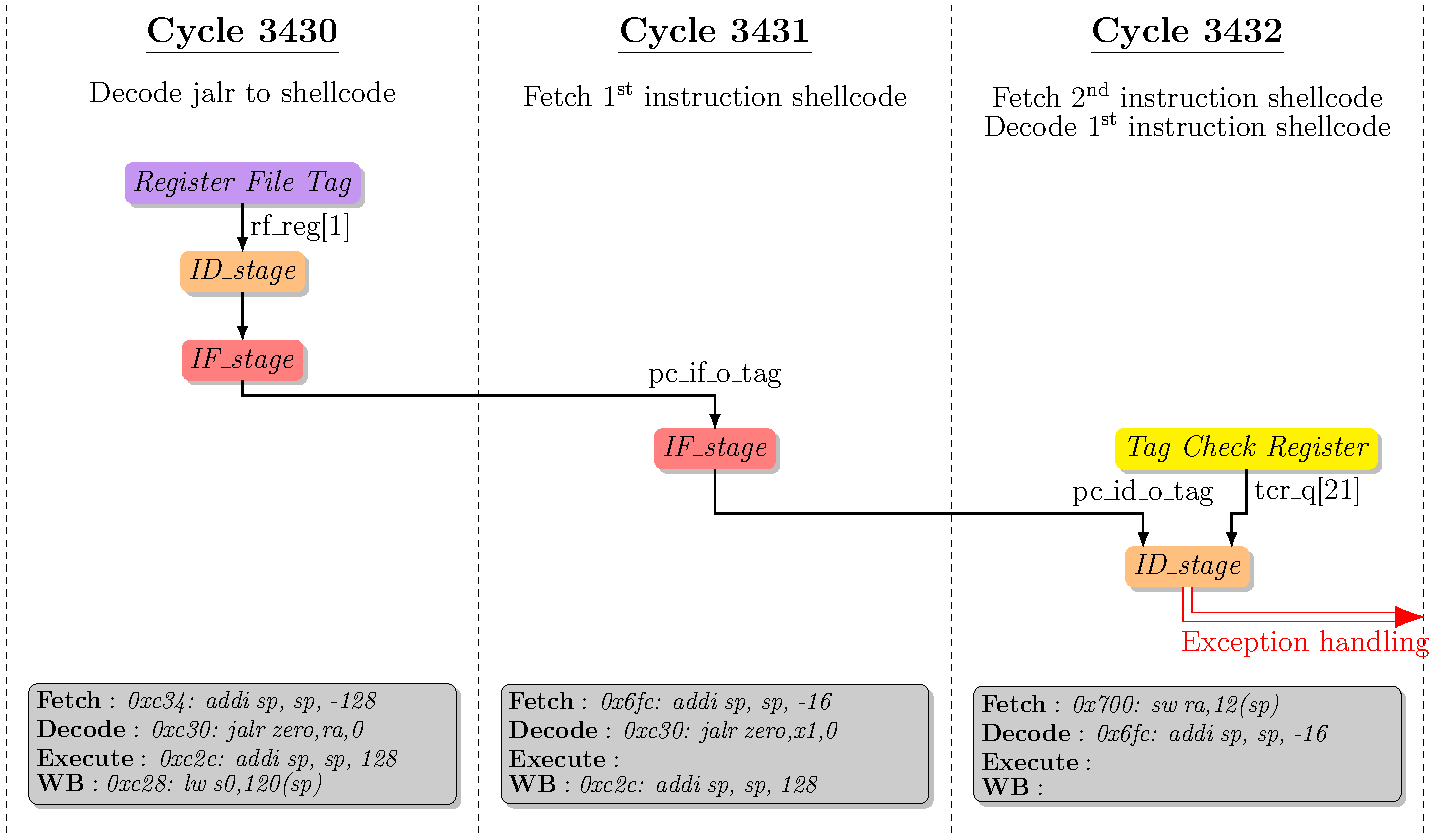
\includegraphics[width=\textwidth]{c3_vulnerabilities_assessment/img/buffer_overflow/bufferOverflowAttack_short.pdf}
    \caption{Tag propagation in a buffer overflow attack}
    \label{fig:study_buffer_overflow_tag_propagation}
\end{figure}

To further study the propagation of the fault, Figure~\ref{fig:buffer_overflow_tag_propagation} illustrates the logical relations between the DIFT-related registers (yellow boxes) and control signals or processor registers (grey boxes) driving the illegal instruction exception signal (red box). This figure does not describe the actual hardware architecture, but highlights the logic path leading to an exception raise. An attacker performing fault injections would like to drive the exception signal to `0' to defeat the D-RI5CY DIFT solution. Figure~\ref{fig:buffer_overflow_tag_propagation} shows that a single fault could lead to a successful injection, since all logic paths are built with \textit{AND} gates. For instance, if register \textit{rf\_reg[1]} is set to 0, the tag will be propagated from \textit{gate 1} to \textit{gate 4}. Then, \textit{gate 5} inputs are \textit{tcr\_q[21]} (i.e., `1') and \textit{pc\_id\_o\_tag} (i.e., `0',  \textit{gate 4} output). Thus, \textit{gate 5} output is driven to `0', disabling the exception. 
From Figure~\ref{fig:buffer_overflow_tag_propagation}, three fault propagation paths can be identified: from \textit{gate 1} to \textit{gate 5} if the fault is injected into \textit{rf\_reg[1]}, from \textit{gate 4} to \textit{gate 5} if a fault is injected into \textit{pc\_if\_o\_tag} and through \textit{gate 5} if a fault is injected into either the \textit{tcr\_q} or \textit{pc\_id\_o\_tag}.
Analysis of Figure~\ref{fig:buffer_overflow_tag_propagation} strengthens the results presented in Table~\ref{tab:end_sim_from_time_fault_register_bo} where \textit{set to 0} and \textit{bit-flip} fault types lead to successful attacks. The root cause is that the propagation paths consist entirely of \textit{AND} gates. 

\begin{figure}[ht]
    \centering
    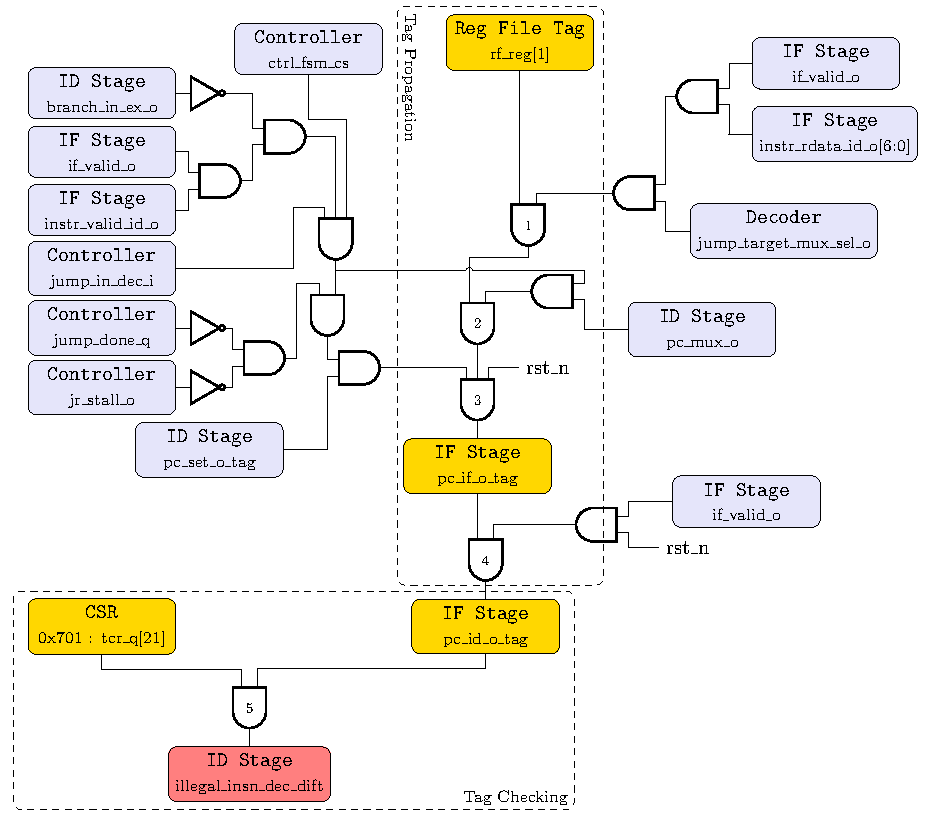
\includegraphics[width=\textwidth]{c3_vulnerabilities_assessment/img/buffer_overflow/arborescence_bufferOverflow.pdf}
    \caption{Logic description of the exception driving in a buffer overflow attack}
    \label{fig:buffer_overflow_tag_propagation}
\end{figure}

%%%%%%%%%%%%%%%%%%%%%%%%%%%%%%%%%%%%%%%%%%
\subsection{Second use case: Format string (WU-FTPd)}
Table~\ref{tab:end_sim_from_time_fault_register_mo} shows that 52 fault injections in 10 DIFT-related registers can lead to a successful attack. 
Furthermore, it shows that 8 different cycles can be targeted for the attack to succeed. 29 successes over 52 are obtained with the \textit{bit-flip} fault type. 
\textit{alu\_operand\_a\_ex\_o\_tag}, \textit{alu\_operand\_b\_ex\_o\_tag} and \textit{alu\_operator\_o\_mode} registers are critical during cycles 52477 and 52478 since they are used for tag propagation related to the C statement \verb|(a-4)|. \textit{alu\_operand\_a\_ex\_o\_tag} and \textit{alu\_operand\_b\_ex\_o\_tag} sequentially store the tag associated to `\verb|a|' while \textit{alu\_operator\_o\_mode} stores the propagation rule according to the TPR configuration (see Table~\ref{tab:tpr}). \textit{regfile\_alu\_waddr\_ex\_o\_tag} stores the destination register index in which the tag resulting from tag propagation should be written.
\textit{check\_s1\_o\_tag} maintains the TCR value from the decode stage to the execution stage, it is compared to the value of the operand tag for tag checking.
\textit{rf\_reg[15]} stores the tag associated with the `\verb|a|' variable.
\textit{store\_dest\_addr\_ex\_o\_tag} maintains the tag of the destination address during a store instruction in the execute stage. 
\textit{use\_store\_ops\_ex\_o} drives a multiplexer to propagate the value stored in \textit{store\_dest\_addr\_ex\_o\_tag} register to the tag checking module.
Finally, faults in \textit{tpr\_q} and \textit{tcr\_q} are successful, since these registers maintain the propagation rules and the security policy configuration. 
The last two registers, \textit{tpr\_q} and \textit{tcr\_q} are critical when we fault the bit 12 of TPR because the load/store mode which is set to \textit{10} but if we change it the propagation policy will change and then the tag will not be propagated as a mode set to \textit{11} will clear the tag. A bit-flip at bit 15 will impact the behaviour as it stores the load/store enable source tag. Finally, bit 20 of TCR store the load/store check destination address tag, which is used when the program wants to store at the address (a-4).

Figure~\ref{fig:study_mem_overwriting_tag_propagation} details the tag propagation in the context of a format string attack case for a non-faulty execution and illustrates the reason behind the sensitivity of registers highlighted in Table~\ref{tab:end_sim_from_time_fault_register_mo}.
Figure~\ref{fig:study_mem_overwriting_tag_propagation} focuses on three clock cycles dedicated to the instruction \verb|sw a4,0(a5)| decoding and execution, which should lead to the storage of the value 224 at address (a-4). 
In cycles 52482 and 52483, \verb|sw a4,0(a5)| is decoded and the source operands tag are retrieved from the tag register file. Particularly, the store destination address is retrieved from \textit{rf\_reg[15]} and stored in register \textit{store\_dest\_addr\_ex\_o\_tag}. In cycle 52484, the destination address of the store operation is computed by the processor Arithmetic Logic Unit (ALU).
In parallel, \textit{alu\_operator\_o\_mode}, \textit{alu\_operand\_a\_ex\_o\_tag}, \textit{alu\_operand\_b\_ex\_o\_tag}, \textit{store\_dest\_addr\_ex\_o\_tag} and \textit{check\_s1\_o\_tag} registers drives the tag computation corresponding to the destination address. 
\textit{use\_store\_ops\_ex\_o} drives a multiplexer to propagate the value stored in \textit{alu\_operand\_a\_ex\_o\_tag} register to the tag checking module. 
\textit{alu\_operand\_a\_ex\_o\_tag} and \textit{alu\_operand\_b\_ex\_o\_tag} sequentially store the tag associated to `\verb|a|' while \textit{alu\_operator\_o\_mode} stores the propagation rule according to the TPR configuration (see Table~\ref{tab:tpr}).
\textit{check\_s1\_o\_tag} maintains the TCR value from the decode stage to the execution stage, it is compared to the value of the operand tag for tag checking.
Then, the store should be executed in the Execute stage. However, the tag associated with the store destination address is set to 1 due to tag propagation (since it is computed from variable `\verb|a|'). 
Since the security policy prohibits the use of data tagged as \textit{untrusted} as a store instruction destination address (\textit{Load/Store Check} field of TCR = 1010), an exception is raised.
\textit{use\_store\_ops\_ex\_o}, highlighted in Table~\ref{tab:end_sim_from_time_fault_register_mo} but not shown in Figure~\ref{fig:study_mem_overwriting_tag_propagation}, drives a multiplexer leading to the propagation of register \textit{store\_dest\_addr\_ex\_o\_tag}.

\begin{landscape}
    \begin{table}[t]
        \footnotesize
        \centering
        \caption{Format string attack: success per register, fault type and simulation time}
        \label{tab:end_sim_from_time_fault_register_mo}
        \setlength{\tabcolsep}{1pt}
        \begin{tabular}{@{}lcccccccccccccccccccccccc@{}}
            \toprule
            & \multicolumn{3}{c}{Cycle 52477} & \multicolumn{3}{c}{Cycle 52478} & \multicolumn{3}{c}{Cycle 52479} & \multicolumn{3}{c}{Cycle 52480} & \multicolumn{3}{c}{Cycle 52481} & \multicolumn{3}{c}{Cycle 52482} & \multicolumn{3}{c}{Cycle 52483} & \multicolumn{3}{c}{Cycle 52484} \\\cmidrule(lr){2-4}\cmidrule(lr){5-7}\cmidrule(lr){8-10}\cmidrule(lr){11-13}\cmidrule(lr){14-16}\cmidrule(lr){17-19}\cmidrule(lr){20-22}\cmidrule(lr){23-25}
            & set0 & set1 & bit-flip & set0 & set1 & bit-flip & set0 & set1 & bit-flip & set0 & set1 & bit-flip & set0 & set1 & bit-flip & set0 & set1 & bit-flip & set0 & set1 & bit-flip & set0 & set1 & bit-flip \\
            \midrule
            alu\_operand\_a\_ex\_o\_tag & \checkmark &  & \checkmark &  &  &  &  &  &  &  &  &  &  &  &  &  &  &  &  &  &  \\
            alu\_operand\_b\_ex\_o\_tag &&&& \checkmark &  & \checkmark &  &  &  &  &  &  &  &  &  &  &  &  &  &  &  &  &  &  \\
            alu\_operator\_o\_mode &\checkmark & \checkmark && \checkmark & \checkmark &  &  &  &  &  &  &  &  &  &  &  &  &  &  &  &  &  &  &  \\
            \rowcolor{LightGray} alu\_operator\_o\_mode[0] &&& \checkmark &&& \checkmark &  &  &  &  &  &&&&&&&&&&&&&  \\
            \rowcolor{LightGray} alu\_operator\_o\_mode[1] &&& \checkmark &&& \checkmark &  &  &  &  &  &&&&&&&&&&&&&  \\
            check\_s1\_o\_tag &&&&  &  &  &  &  &  &  &  &  &  &  &  &  &  &  &  &  &  & \checkmark &  & \checkmark \\
            regfile\_alu\_waddr\_ex\_o\_tag[1] &&&&  &  &  &  &  &  &  &  &  &  &  & \checkmark &  &  &  &  &  &  &  &  &  \\
            rf\_reg[15] &&&&  &  &  &  &  &  &  &  &  &  &  &  & \checkmark &  & \checkmark & \checkmark &  & \checkmark &  &  &  \\
            store\_dest\_addr\_ex\_o\_tag &&&&  &  &  &  &  &  &  &  &  &  &  &  &  &  &  &  &  &  & \checkmark &  & \checkmark \\
            tcr\_q & \checkmark &&& \checkmark &  &  & \checkmark &  &  & \checkmark &  &  & \checkmark &  &  & \checkmark &  &  & \checkmark &  &  &  &  &  \\
            \rowcolor{LightGray} tcr\_q[20] &&& \checkmark &&& \checkmark &&& \checkmark &&& \checkmark &&& \checkmark &&& \checkmark &&& \checkmark &&&  \\
            tpr\_q && \checkmark &&  & \checkmark &  &  & \checkmark &  &  & \checkmark &  &  & \checkmark &  &  &  &  &  &  &  &  &  &  \\
            \rowcolor{LightGray} tpr\_q[12] &&& \checkmark &&& \checkmark &&& \checkmark &&& \checkmark &&& \checkmark &  &  &&&&&&&  \\
            \rowcolor{LightGray} tpr\_q[15] &&& \checkmark &&& \checkmark &&& \checkmark &&& \checkmark &&& \checkmark &  &  &&&&&&&  \\
            use\_store\_ops\_ex\_o &&&&  &  &  &  &  &  &  &  &  &  &  &  &  &  &  &  &  &  & \checkmark &  & \checkmark \\
            \bottomrule
        \end{tabular}
    \end{table}
\end{landscape}

 \begin{figure}[ht]
    \centering
    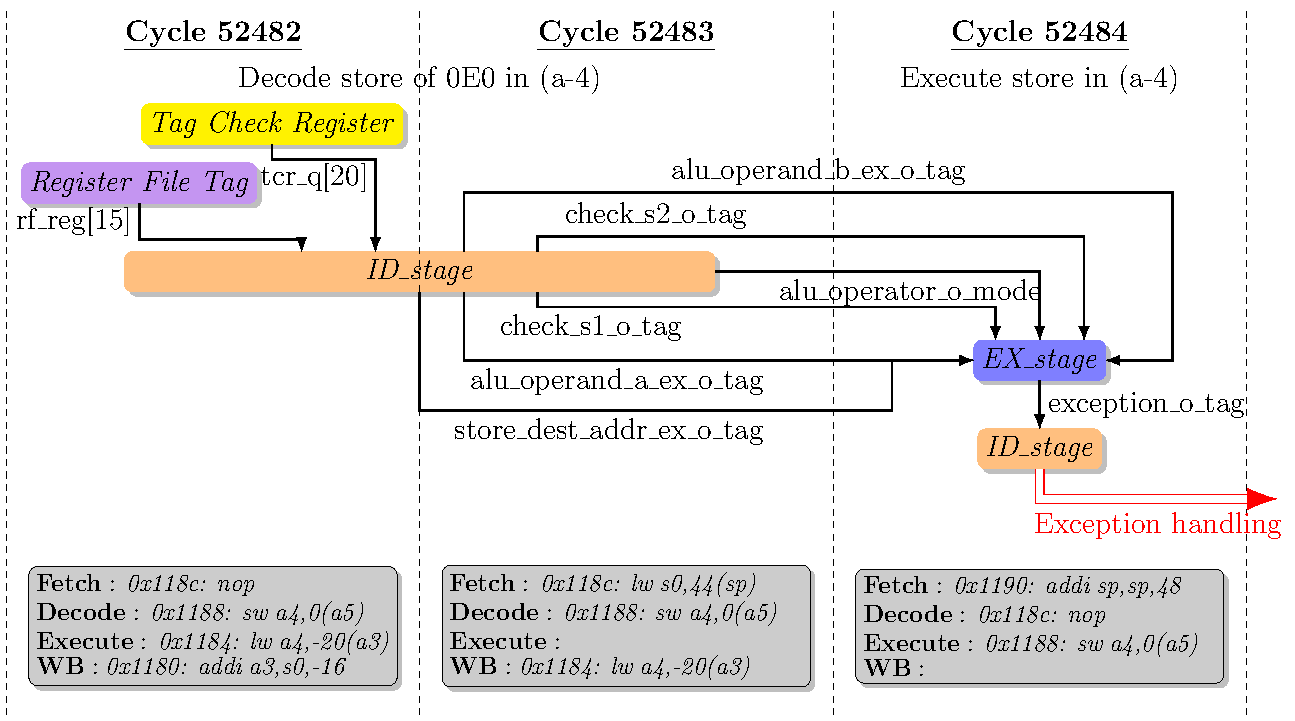
\includegraphics[width=\linewidth]{c3_vulnerabilities_assessment/img/wuftpd/full_ftpd_short.pdf}
    \caption{Tag propagation in a format string attack}
    \label{fig:study_mem_overwriting_tag_propagation}
 \end{figure}

To further study the propagation of the fault, Figure~\ref{fig:mem_overwriting_tag_propagation} illustrates the logical relations between the DIFT-related registers (yellow boxes) and control signals or processor registers (gray boxes) driving the illegal instruction exception signal (red box) for the second use case. 
Figure~\ref{fig:mem_overwriting_tag_propagation} shows that a single fault could lead to a successful injection, since all logic paths are built with \textit{AND} gates. For instance, if register \textit{rf\_reg[15]} is set to 0, this tag value will be propagated from \textit{gate 8} to \textit{gate 11} and to \textit{mux 12}. Then, since \textit{mux 12} output drives one \textit{gate 3} input, \textit{gate 3} output is driven to `0', the exception is disabled. 
From Figure~\ref{fig:mem_overwriting_tag_propagation}, seven fault propagation paths can be identified: 
from \textit{gate 1} to \textit{gate 3} if the fault is injected into \textit{tcr\_q[20]},
through \textit{gate 3} if a fault is injected into \textit{check\_s1\_o\_tag},
from \textit{gate 4} or \textit{gate 5} to \textit{gate 3} if a fault is injected into \textit{alu\_operand\_b\_ex\_o\_tag} or \textit{alu\_operand\_a\_ex\_o\_tag},
from \textit{mux 6} to \textit{gate 3} if a fault is injected into \textit{alu\_operator\_o\_mode},
from \textit{mux 7} to \textit{gate 3} if a fault is injected into \textit{regfile\_alu\_waddr\_ex\_o\_tag},
from \textit{gate 8} to \textit{gate 3} if a fault is injected in the tag register file (i.e., register \textit{rf\_reg[15]}) and
from \textit{mux 11} to \textit{gate 3} if a fault is injected in either \textit{store\_dest\_addr\_ex\_o\_tag} or \textit{use\_store\_ops\_ex\_o}.
Analysis of Figure~\ref{fig:mem_overwriting_tag_propagation} reinforces the results presented in Table~\ref{tab:end_sim_from_time_fault_register_mo} where \textit{set to 0} and \textit{bit-flip} fault types lead to successful attacks. As with the first use case, the main cause is that the propagation paths are fully made of \textit{AND} gates. As shown in Table~\ref{tab:end_sim_from_time_fault_register_mo} \textit{alu\_operator\_o\_mode} register is sensitive to \textit{set to 0} and \textit{set to 1} fault types. Indeed, this register determines the tag propagation according to TPR. The tag propagation is disabled when a TPR field is set to `00' and the output tag is set to 0 (i.e., trusted) when a TPR field is set to `11'. 

 \begin{figure}[ht]
    \centering
    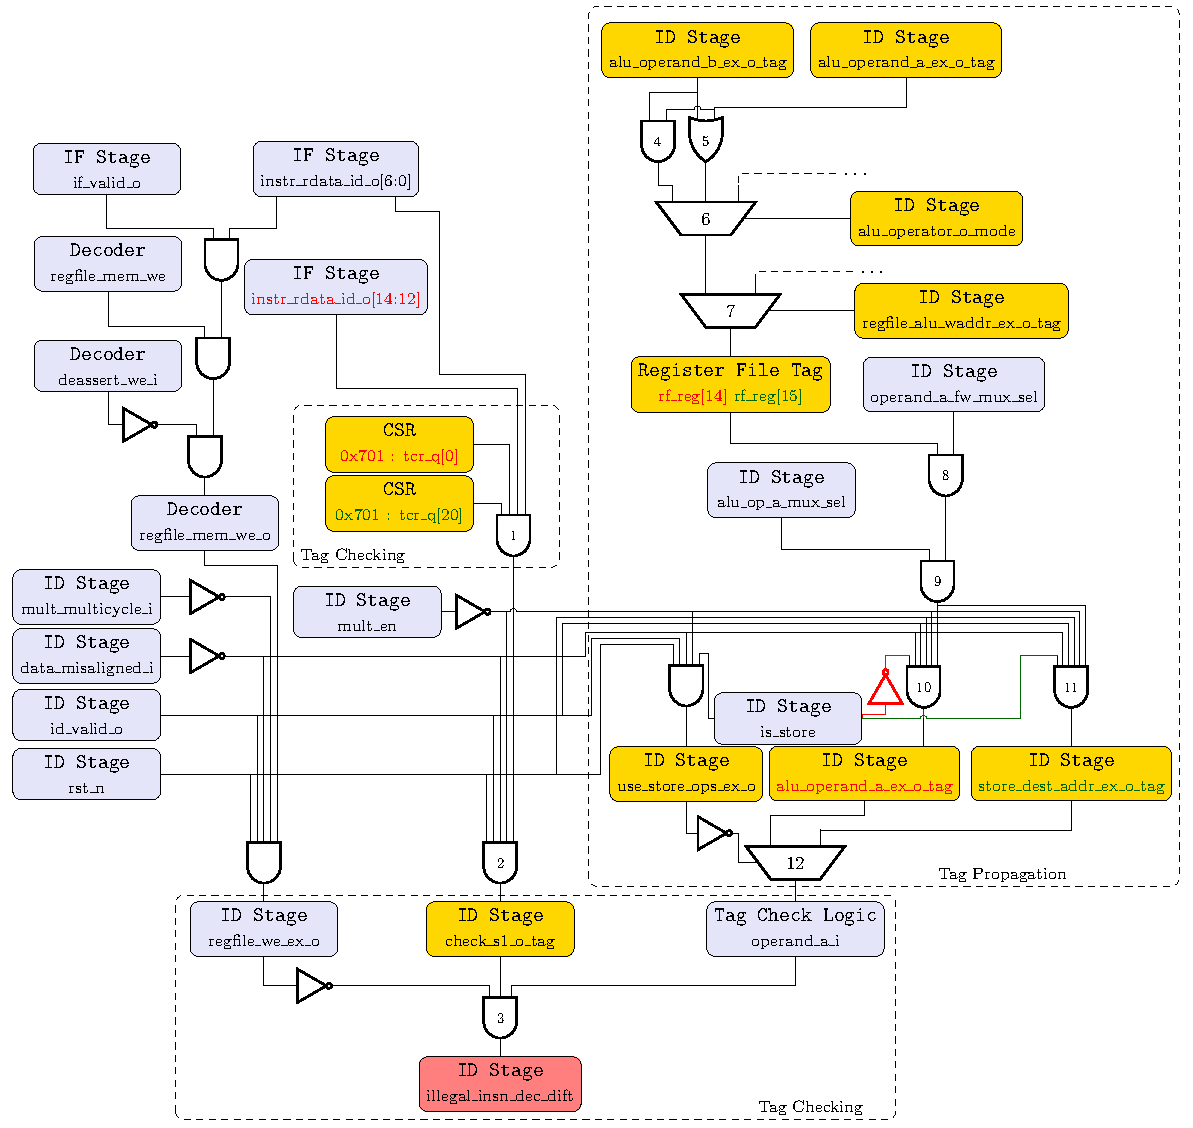
\includegraphics[width=\linewidth]{c3_vulnerabilities_assessment/img/wuftpd/arborescence_v3_wuftpd.pdf}
    \caption{Logic description of the exception driving in a format string attack}
    \label{fig:mem_overwriting_tag_propagation}
 \end{figure}


%%%%%%%%%%%%%%%%%%%%%%%%%%%%%%%%%%%%%%%%%%
\subsection{Third use case: Compare/Compute}
Table~\ref{tab:end_sim_from_time_fault_register_secpoV3} shows that 19 fault injections in 6 DIFT-related registers can lead to a successful attack. Furthermore, it shows that 4 different cycles can be targeted for the attack to succeed. The highest success rate is obtained with the \textit{bit-flip} fault type, with 10 successes over 19. 
Faults in \textit{rf\_reg[14]} and \textit{alu\_operand\_a\_ex\_o\_tag} are successful, since these registers store the tag associated to variable \verb|a| during tag propagation. \textit{check\_s1\_o\_tag} maintains one configuration bit from \textit{tcr\_q} during tag checking.
\textit{use\_store\_ops\_ex\_o} drives a multiplexer to propagate the value stored in \textit{alu\_operand\_a\_ex\_o\_tag} register to the tag checking module. 
For this case, the critical registers can be found in previous case, \textit{alu\_operand\_a\_ex\_o\_tag} propagate the tag of the tagged variable in the code (variable \verb|a|). 
Finally, observations for both \textit{tpr\_q} and \textit{tcr\_q} are similar than for previous case studies. 
Finally, faults in \textit{tpr\_q} and \textit{tcr\_q} are successful, since these registers maintain the propagation rules and the security policy configuration. 

\begin{table}[t]
   \small
   \centering
   \caption{Compare/compute: number of faults per register, per fault type and per cycle}
   \label{tab:end_sim_from_time_fault_register_secpoV3}
   \setlength{\tabcolsep}{4pt}
   \begin{tabular}{@{}lcccccccccccc@{}}
        \toprule
        & \multicolumn{3}{c}{Cycle 832} & \multicolumn{3}{c}{Cycle 833} & \multicolumn{3}{c}{Cycle 834} & \multicolumn{3}{c}{Cycle 835} \\\cmidrule(lr){2-4}\cmidrule(lr){5-7}\cmidrule(lr){8-10}\cmidrule(lr){11-13}
        & set0 & set1 & bit-flip & set0 & set1 & bit-flip & set0 & set1 & bit-flip & set0 & set1 & bit-flip \\
        \midrule
        alu\_operand\_a\_ex\_o\_tag &  &  &  &  &  &  &  &  &  & \checkmark &  & \checkmark \\
        check\_s1\_o\_tag &  &  &  &  &  &  &  &  &  & \checkmark &  & \checkmark \\
        rf\_reg[14] &  &  &  & \checkmark &  & \checkmark & \checkmark &  & \checkmark &  &  &  \\
        tcr\_q & \checkmark &  &  & \checkmark &  &  & \checkmark &  &  &  &  &  \\
        \rowcolor{LightGray} tcr\_q[0] &&& \checkmark &&& \checkmark &&& \checkmark &&&  \\
        tpr\_q &  & \checkmark &  &  &  &  &  &  &  &  &  &  \\
        \rowcolor{LightGray} tpr\_q[12] &&& \checkmark &  &  &&&&&&&  \\
        \rowcolor{LightGray} tpr\_q[15] &&& \checkmark &  &  &&&&&&&  \\
        use\_store\_ops\_ex\_o &  &  &  &  &  &  &  &  &  &  & \checkmark & \checkmark \\
        \bottomrule
    \end{tabular}
\end{table}

Figure~\ref{fig:study_attack_propag_v3_tag_propagation} focuses on the three cycles, represented in red, corresponding to \verb|add a5,a4,a5| instruction (C statement \verb|(a+b)|) decoding and execution in the context of the third use case. 
The instruction \verb|add a5,a4,a5| is in decode stage during cycles 833 and 834 and the tag associated to the untrusted variable \verb|a| is retrieved from \textit{rf\_reg[14]}. In cycle 835, this addition is executed. In parallel, variable \verb|a| tag is propagated to the tag check logic unit, which behaviour is driven by \textit{check\_s1\_o\_tag} through \textit{alu\_operand\_a\_ex\_o\_tag}. Since the V2 security policy prohibits the use of untrusted data as a source operand of an arithmetic operation, an exception is raised. 

Figure~\ref{fig:study_attack_propag_v3_tag_propagation} illustrates the reason behind the sensitivity of registers \textit{rf\_reg[14]}, \textit{alu\_operand\_a\_ex\_o\_tag} and \textit{check\_s1\_o\_tag} highlighted in Table~\ref{tab:end_sim_from_time_fault_register_secpoV3}.
Note that \textit{use\_store\_ops\_ex\_o} does not appear in Figure~\ref{fig:study_attack_propag_v3_tag_propagation}. This register drives a multiplexer leading to tag propagation presented in Figure~\ref{fig:study_attack_propag_v3_tag_propagation}.

\begin{figure}[ht]
    \centering
    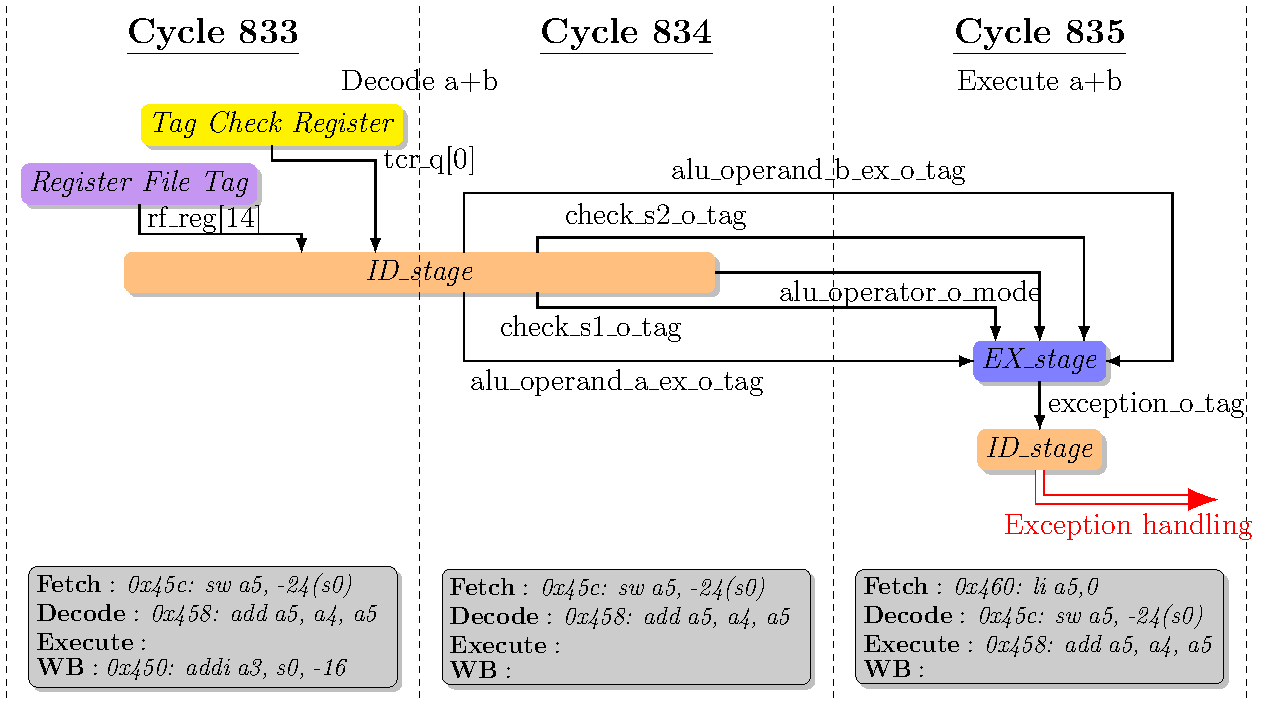
\includegraphics[width=\linewidth]{c3_vulnerabilities_assessment/img/comp_compu/attaquePropag_v3_short.pdf}
    \caption{Tag propagation in a computation case with the compare/compute use case}
    \label{fig:study_attack_propag_v3_tag_propagation}
\end{figure}

To further study the faults' propagation, Figure~\ref{fig:attack_propag_v3_tag_propagation} illustrates the logical relations between the DIFT-related registers (yellow boxes) and control signals or processor registers (gray boxes) driving the illegal instruction exception signal (red box).
Figure~\ref{fig:attack_propag_v3_tag_propagation} shows that a single fault could lead to a successful injection, since all logic paths are built with \textit{AND} gates. For instance, if register \textit{rf\_reg[14]} is set to 0, the tag will be propagated from \textit{gate 8} to \textit{gate 10} and to \textit{mux 12}. Then, since \textit{mux 12} output drives one \textit{gate 3} output, the exception is disabled.
From Figure~\ref{fig:attack_propag_v3_tag_propagation}, seven fault propagation paths can be identified. We won't go into detail here about the seven different paths, as they were mentioned in case 2, bearing in mind that colour differentiation must be taken into account (for example: \textit{alu\_operand\_a\_ex\_o\_tag} instead of \textit{store\_dest\_addr\_ex\_o\_tag}
from \textit{gate 1} to \textit{gate 3} if the fault is injected into \textit{tcr\_q[0]},
through \textit{gate 3} if a fault is injected into \textit{check\_s1\_o\_tag},
from \textit{gate 4} or \textit{gate 5} to \textit{gate 3} if a fault is injected into \textit{alu\_operand\_b\_ex\_o\_tag} or \textit{alu\_operand\_a\_ex\_o\_tag},
from \textit{mux 6} to \textit{gate 3} if a fault is injected into \textit{alu\_operator\_o\_mode},
from \textit{mux 7} to \textit{gate 3} if a fault is injected into \textit{regfile\_alu\_waddr\_ex\_o\_tag}, from \textit{gate 8} to \textit{gate 3} if a fault is injected into \textit{rf\_reg[14]}, and
from \textit{mux 11} to \textit{gate 3} if a fault is injected into either \textit{alu\_operand\_a\_ex\_o\_tag} or \textit{use\_store\_ops\_ex\_o}.
Analysis of Figure~\ref{fig:attack_propag_v3_tag_propagation} supports the results presented in Table~\ref{tab:end_sim_from_time_fault_register_secpoV3} where \textit{set to 0} and \textit{bit-flip} fault types lead to successful attacks. As with first and second use cases, the main reason is that the propagation paths are built entirely from \textit{AND} gates.

\begin{figure}[ht]
    \centering
    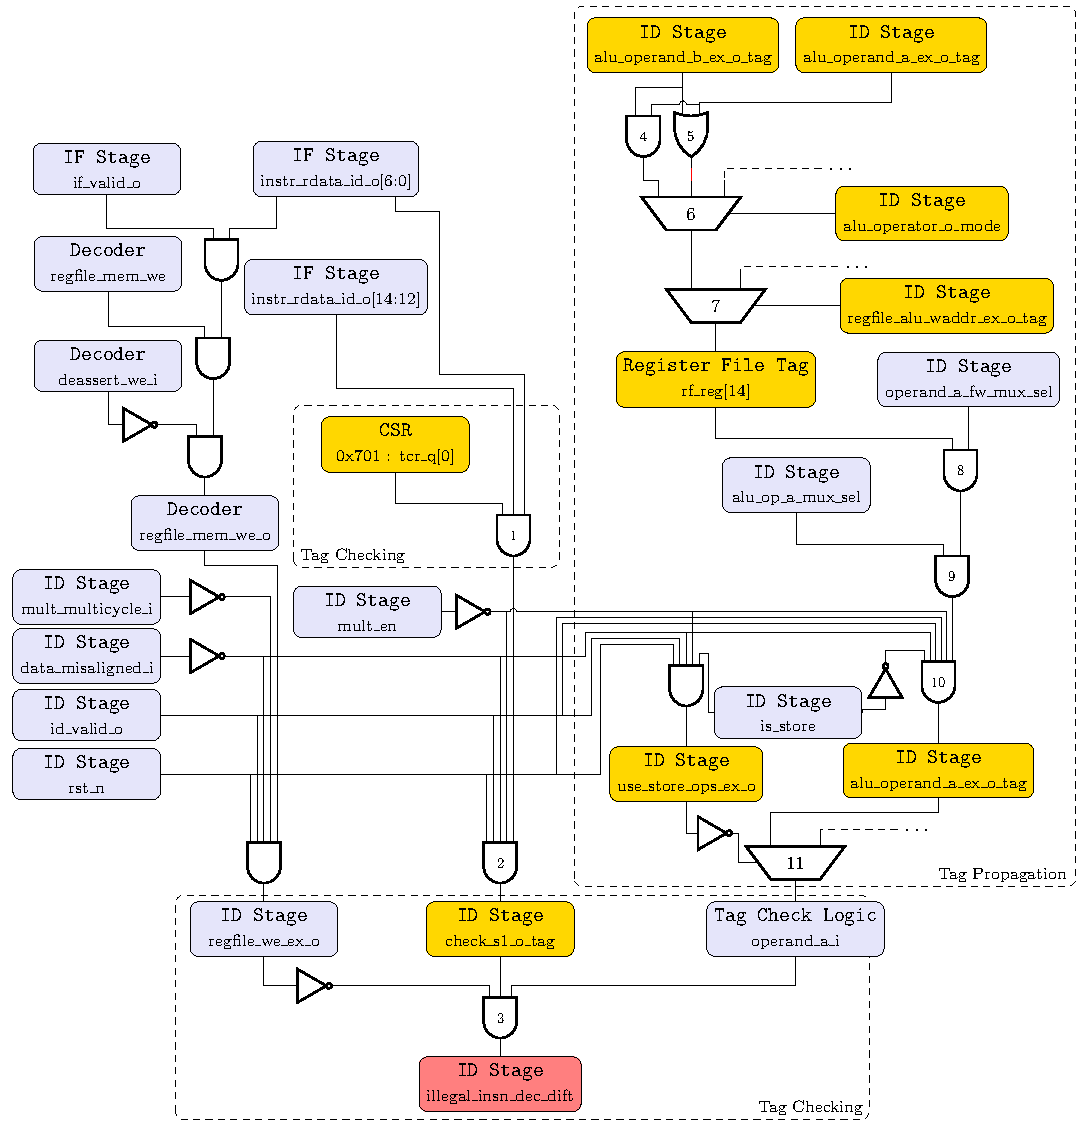
\includegraphics[width=\textwidth]{c3_vulnerabilities_assessment/img/comp_compu/arborescence_propagation.pdf}
    \caption{Logic representation of tag propagation in a computation case}
    \label{fig:attack_propag_v3_tag_propagation}
\end{figure}


%%%%%%%%%%%%%%%%%%%%%%%%%%%%%%%%%%%%%%%%%%%%%%%%%%%%%%%%%%%%%%%%%%%%%%%%%%%%%%%%%%%%%%%%%%%%%%%
\section{Summary}
In this chapter, we described the processor we focus on, with its implementation of a hardware in-core DIFT. We described how it works and how to use the DIFT mechanism with the default configuration. Then, we described the different use cases we choose to work with, in order to analyse the DIFT behaviour and assess it against fault injection attacks. Finally, we presented the vulnerability assessment on these use cases using the D-RI5CY security mechanism. We have shown that this DIFT implementation is vulnerable to FIA within different registers depending on the fault model and depending on the application, as different paths are used and so different registers are going to be critical.
%%%%%%%%%%%%%%%%%%%%%%%%%%%%%%%%%%%%%%%%%%%%%%%%%%%%%%%%%%%%%%%%%%%%%%%%%%%%%%%%%%%%%%%%%%%%%%%